% =============================================================================
% §4 Experiments and Results (~3.0 pages)
% =============================================================================
\section{Experiments and Results}
\label{sec:experiments}

% =============================================================================
\subsection{Setup}
\label{sec:setup}

% Table 1 (tab:main-eff) declared inside §4.1 so it is queued while the Setup
% page composes and its full-width table*[t] float lands at the top of the next
% page, alongside the §4.2 Main results discussion (dblfloatfix).
\begin{table*}[!t]
\centering\small
\setlength{\tabcolsep}{7pt}
\begin{tabular}{@{}lccc@{}}
\toprule
 & SkillsBench & GDPVal & QwenClawBench \\
Cell & \scriptsize no-skill$\to$skill & \scriptsize no-skill$\to$skill & \scriptsize no-skill$\to$skill \\
\midrule
OpenClaw $\times$ Q-27B    & $8.8 \to 13.0$  & $81.2 \to 83.1$ & $65.2 \to 66.7$ \\
OpenClaw $\times$ Q-397B   & $11.1 \to 16.9$ & $82.2 \to 84.0$ & $65.7 \to 67.0$ \\
Raven $\times$ Q-27B       & $10.0 \to 16.5$ & $82.6 \to 83.8$ & $66.9 \to 70.8$ \\
Raven $\times$ Q-397B      & $9.2 \to \mathbf{22.6}$ & $84.0 \to 85.2$ & $68.8 \to 73.2$ \\
\midrule
Pooled $\Delta$ & $+7.5{\pm}2.3$ ($z{=}3.2$) & $+1.51{\pm}0.49$ ($z{=}3.1$) & $+2.79{\pm}0.70$ ($z{=}4.0$) \\
\bottomrule
\end{tabular}
\caption{Main results: absolute performance per cell and
benchmark, no-skill baseline $\to$ SkillCorpus condition.
SkillsBench reports pass@1 averaged over three runs
(\%, $n{=}87$ tasks, the $4$ that do not build scored as
failures).  GDPVal reports
the mean LLM-judge reward (3-rep) over all $220$ tasks.
QwenClawBench reports the mean hybrid
score (automated checks and an LLM judge), 3-rep mean.  Rewards are
on $[0,1]$, shown $\times 100$.  Per-cell gains are visualised in
Figure~\ref{fig:main_heatmap}.
The bottom row gives the pooled $\Delta$ across the four cells,
with a task-clustered standard error over $n{=}87/220/100$ tasks
and two-sided $z{=}\Delta/\mathrm{SE}$.}
\label{tab:main-eff}
\end{table*}

\paragraph{Benchmarks, harnesses, and backbones.}
We evaluate on three third-party agent benchmarks, chosen
because frontier LLMs do not saturate them and their domain
coverage is complementary.  SkillsBench \citep{SkillsBench2026}
contributes $87$ deterministic-verifier tasks across $8$
domains and is the closest direct analog to our setting.
GDPVal \citep{OpenAIGDPVal2025} contributes $220$ real-world
economic tasks that span legal, financial, design, and writing
work.  QwenClawBench \citep{QwenClawBench2026} adds $100$ agent
tasks across $8$ domains drawn from a real-user task
distribution.
In total the evaluation covers $407$ tasks spanning $26$
domain labels (Appendix~\ref{app:coverage},
Figure~\ref{fig:domain_coverage}).
We use two
open-source \texttt{SKILL.md}-conformant agent harnesses,
OpenClaw~\citep{OpenClaw2025} and Raven~\citep{Raven2026},
developed independently, paired with two open backbones that
span the lightweight-to-large range, Qwen3.5-27B (Q-27B) and
Qwen3.5-397B-A17B-GPTQ-Int4 (Q-397B), yielding four
(harness, backbone) cells.  A frontier-model robustness check on
Claude~Opus~4.7 verifies that the effect
is not specific to the open backbones.

\paragraph{Configurations, inference, and metrics.}
Each cell is evaluated under a no-skill baseline and under
SkillCorpus paired with our retrieval-and-selection stack
(\S\ref{sec:retrieval}), whose standalone retrieval performance
is reported in \S\ref{sec:retrieval-perf}.  The per-cell
$\Delta$ therefore measures the end-to-end pipeline effect.  All
runs use each backbone's API-default
inference configuration.  The Qwen models run greedy decoding
with their default context and tool-use template, and Opus~4.7
runs at its default thinking effort.  \ifarxiv
Both conditions in a cell
share the same setting, so the reported within-cell $\Delta$ is
unaffected by inference effort and remains valid even though our
vendor-default absolute baselines are not directly comparable to
published leaderboard numbers obtained under other
configurations.
\else
Both conditions in a cell share the same setting, so the within-cell
$\Delta$ stays valid even though our vendor-default absolute
baselines are not comparable to published leaderboard numbers.
\fi  For SkillsBench we report the binary
pass rate over all $87$ tasks, scoring the $4$ that
do not build in our environment as failures in both
conditions.  For GDPVal and QwenClawBench we report the mean
continuous reward, both on $[0,1]$ with $\Delta$ in percentage
points.  GDPVal is scored by a GPT-4o judge, from a different
model family than our Qwen and Opus backbones, and QwenClawBench
by its official grading configuration combining automated checks
with an LLM judge \citep{QwenClawBench2026}.  The main grid holds $24$ configurations, the four cells
evaluated on three benchmarks under both conditions, each
averaged over three runs.  With the two-condition single-run
frontier check, this comes to $74$ end-to-end runs.
Appendix~\ref{app:compute} reports the ingest and evaluation
compute.

% =============================================================================
\subsection{Main results}
\label{sec:main-results}

\ifarxiv
Table~\ref{tab:main-eff} reports the absolute performance of
the no-skill baseline and the SkillCorpus condition (the corpus
with our retrieval-and-selection stack) for each of the four
(harness, backbone) cells on each benchmark.  The per-cell
gains ($\Delta$) and their per-cell means are visualised in
Figure~\ref{fig:main_heatmap}.
\else
Table~\ref{tab:main-eff} reports absolute performance for the
no-skill baseline and SkillCorpus across the four cells and three
benchmarks, with the per-cell gains ($\Delta$) and their means in
Figure~\ref{fig:main_heatmap}.
\fi

\begin{figure}[!t]
\centering
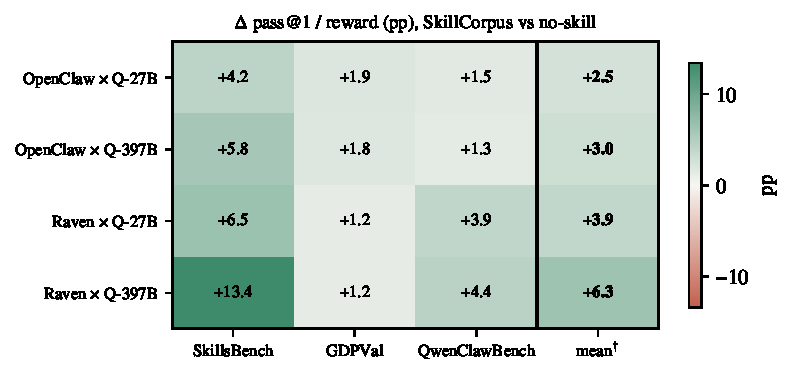
\includegraphics[width=\columnwidth]{figures/fig_main_heatmap.pdf}
\caption{Per-cell, per-benchmark $\Delta$ (pp) computed from
the absolute values in Table~\ref{tab:main-eff}.  Green =
positive, red = negative.
$^{\dagger}$Mean over the three benchmarks.}
\label{fig:main_heatmap}
\end{figure}

% SkillsBench column = get_result_all.py 3-rep mean over jobs_6.3/6.6/6.8,
% 87-denom (4 unbuilt=fail); Δ mean±SE (per cell, n=87):
% oc27 +4.2±2.7, oc397 +5.7±3.1, ec27 +6.5±3.0, ec397 +13.4±3.1;
% pooled +7.47, task-clustered SE 2.35 (z=3.2). (Replaces old +8.4
% 8way_summary headline, 2026-06-16.)
% SE convention = task-clustered: per-task Δ averaged over 4 cells, then
% std/√n over n tasks (NOT pooled cell-task n=4×tasks, which understates SE).
% GDPVal column = FINAL 220 full-set 3-rep mean (0616 regrade,
% analysis_cache/gdpval_percase_full.csv); retry-dedup = keep-original
% (per (task,round) keep __trial_1, drop _retry*; matches oc cells which have
%  no retries; 2026-06-25). Δ: oc27 +1.9, oc397 +1.8, ec27 +1.2, ec397 +1.2;
% pooled +1.51, SE 0.49 (z=3.1). ec base lifted ~2pp vs old pool-all conv.
% (ec27 80.5->82.6, ec397 81.9->84.0) since originals score above retries.
% (regrade 0616 lifted mis-graded skill-arm rows upward, all on skill arm;
%  no-skill arm aggregate unchanged. Confirmed real grader errors.)
% QwenClawBench column = FINAL C (3-round splice, patched gate + reference-usage
% prompt, 0616). Δ: oc27 +1.5, oc397 +1.4,
% ec27 +3.9, ec397 +4.4; pooled +2.79, task-clustered SE 0.70 (z=4.0).
On SkillsBench, which has a
published oracle baseline \citep{SkillsBench2026}, all four
open-backbone cells show positive $\Delta$ averaging
$+7.5$\,pp over three runs, from $+4.2{\pm}2.7$ on the weakest
cell to $+13.4{\pm}3.1$ on the strongest
(Raven~$\times$~Q-397B), with an aligned $+8.0$\,pp on the
Claude~Opus~4.7 frontier check.  In one
run the strongest cell rescues $19$
baseline-failing tasks while breaking $2$ (exact McNemar test,
$p{<}0.001$).  No cell shows a net-negative mean, so at the cell-mean level the
corpus behaves as a no-harm attachment whose upside varies by
cell, even though individual tasks can still regress
(\S\ref{sec:negative}).

\paragraph{Consistent positive effect across benchmarks.}
\ifarxiv
We quantify the effect at the benchmark level by averaging each
task's paired delta across the four cells and computing a
task-clustered standard error, $\mathrm{SE}=\mathrm{std}/\sqrt{n}$
over the $n$ tasks, so that repeated measurements of the same task
across cells are not treated as independent observations.  This is
the more conservative of two reasonable clusterings.  Pooling the
cell--task deltas as independent observations would roughly halve
the standard errors, and the positive effect holds
under either choice.
\else
We quantify the effect at the benchmark level by averaging each
task's paired delta across the four cells and computing a
task-clustered standard error ($\mathrm{SE}=\mathrm{std}/\sqrt{n}$
over the $n$ tasks), so repeated measurements of the same task are
not treated as independent.  This is the more conservative
clustering, and pooling the cell--task deltas would roughly halve
the SEs, but the effect holds either way.
\fi
All
three benchmarks show a consistent positive effect, each
exceeding twice its standard error (bottom row of
Table~\ref{tab:main-eff}).
\ifarxiv
Effect size broadly tracks the headroom a benchmark leaves.
SkillsBench starts near a $10\%$ no-skill baseline and
gains the most, and within it the low-baseline
Industrial~\&~Physical category gains most ($+45.5$\,pp), whereas
GDPVal and QwenClawBench start at $65$--$85\%$ and gain less, where
ceiling effects and judge noise both bound the realisable gain.  Per-task repetition noise is large
on the high-baseline benchmarks, with per-task reward standard
deviations of $20$--$27$\,pp on GDPVal, so most individual cells
are not separately distinguishable from zero.
\else
Effect size broadly tracks the headroom a benchmark leaves.
SkillsBench starts near a $10\%$ no-skill baseline and gains the
most, and within it the low-baseline Industrial~\&~Physical
category gains most ($+45.5$\,pp), whereas GDPVal and QwenClawBench
start at $65$--$85\%$ and gain less, bounded by ceiling effects and
judge noise.  Per-task reward SDs of $20$--$27$\,pp on GDPVal leave
most individual cells indistinguishable from zero.
\fi  \ifarxiv
We do
not observe the negative tail that \citet{SkillsBench2026} reports
for hand-attached skills, nor the failure to improve over a
no-skill baseline reported for uncurated community libraries
\citep{SkillFlow2026,UCSBSkillsWild2026}, a difference consistent with the release gates that
remove the low-quality mass driving them.
\else
We see neither the negative tail \citet{SkillsBench2026} reports for
hand-attached skills nor the no-improvement result for uncurated
libraries \citep{SkillFlow2026,UCSBSkillsWild2026}, consistent with
our release gates removing the low-quality mass driving them.
\fi  Raven outgains OpenClaw on SkillsBench and QwenClawBench
across both backbones.  On GDPVal neither harness leads, as the
gains there are small and individually not significant.  The harness
thus shapes how much of the gain is realised
(\S\ref{sec:discussion}).

% =============================================================================
\subsection{Frontier robustness check}
\label{sec:frontier}
The four main-grid cells span the open capability range
(Q-27B, Q-397B).  To verify that the pipeline's effect is not
specific to this range, we add a single-cell check on
Claude~Opus~4.7 on SkillsBench (OpenClaw harness) under the same
two-condition protocol.  Opus~4.7 reaches a $39.1\%$ no-skill baseline on the $87$-task
set, and adding SkillCorpus shifts pass@1 to $47.1\%$, a $\Delta$
of $+8.0$\,pp.  \ifarxiv
Although the Opus baseline is several times the
open-backbone baselines, its gain is of the same order as the
open-backbone cross-cell mean, indicating that stronger frontier
models have not made an external curated skill pipeline redundant
on this benchmark.  We treat this as a robustness check, and a
broader frontier grid is left for follow-up work.
\else
Although the Opus baseline is several times the open-backbone
baselines, its gain is of the same order as the open-backbone mean,
so stronger frontier models have not made an external curated skill
pipeline redundant here.  A broader frontier grid is left for
follow-up.
\fi

% --------------------------------------------------------- 4.2.Y retrieval-perf
\subsection{Standalone retrieval}
\label{sec:retrieval-perf}
End-to-end $\Delta$ entangles corpus quality with retrieval
quality.  We additionally evaluate the recall-and-rerank stack as a
standalone retrieval system on the SkillRouter Easy and Hard
tiers \citep{SkillRouter2026} and on our SkillCorpus pool, a
75-task core SkillsBench set.  Figure~\ref{fig:retrieval_perf}
reports Hit@1 and Recall@10 across the three pools, with full
setup and per-method results in Appendix~\ref{app:retrieval-perf}.

\begin{figure}[!ht]
\centering
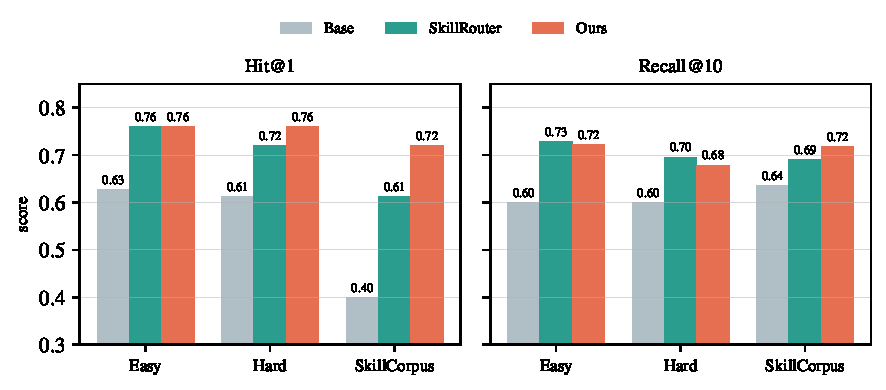
\includegraphics[width=\columnwidth]{figures/fig_retrieval_perf.pdf}
\caption{Standalone retrieval performance of \textsc{Base},
\textsc{SkillRouter}, and our fine-tuned stack on the three
candidate pools (Hit@1 / Recall@10, exact numbers in
Table~\ref{tab:skill_routing_performance}).}
\label{fig:retrieval_perf}
\end{figure}
Despite being trained on a different pool, our stack matches
\textsc{SkillRouter} on the Easy tier and exceeds it on the Hard
tier, staying within $1.7$\,pp on Recall@10.  On SkillCorpus it
outperforms \textsc{SkillRouter} by $+10.7$\,pp Hit@1 and
$+2.7$\,pp Recall@10, a margin that partly reflects the matched
train and evaluation distribution and the ground-truth skills
injected into this pool (Appendix~\ref{app:retrieval-perf}).

% =============================================================================
\subsection{Ablation: corpus and retrieval}
\label{sec:ablation}

To gauge how much of the gain comes from corpus curation versus
the fine-tuned retrieval stack, we lesion each in turn on the
strongest cell (Raven~$\times$~Q-397B, SkillsBench).  Replacing
our retrieval stack with off-the-shelf Qwen3 embedding and
reranking models lowers pass@1 from $22.6\%$ to $13.8\%$, and
replacing the filtered corpus with the $\sim$$821{,}000$-file raw
crawl lowers it to $14.9\%$ (Table~\ref{tab:ablation}).  \ifarxiv
Both remain well
above the $9.2\%$ no-skill baseline yet well below the full
pipeline, so curation and retrieval each contribute and neither
alone accounts for the full gain, though the end-to-end $\Delta$
also folds in the LLM rewriter/selector layer that this ablation
does not isolate.  These are single-run numbers
with inter-arm gaps of only a few tasks, so we read them as
directional and leave a repeated ablation to future work.
\else
Both remain well above the $9.2\%$ no-skill baseline yet below the
full pipeline, so curation and retrieval each contribute and neither
alone accounts for the full gain, which also folds in the LLM
rewriter/selector layer this ablation does not isolate.  These
single-run numbers have inter-arm gaps of only a few tasks, so we
read them as directional and leave a repeated ablation to future
work.
\fi

\begin{table}[!ht]
\centering\small
\setlength{\tabcolsep}{6pt}
\begin{tabular}{@{}llcc@{}}
\toprule
Corpus & Retrieval stack & pass@1 & $\Delta$ \\
\midrule
\multicolumn{2}{@{}l}{No-skill baseline} & $9.2$ & --- \\
\midrule
Filtered  & Fine-tuned (ours)   & $\mathbf{22.6}$ & $\mathbf{+13.4}$ \\
Filtered  & Off-the-shelf Qwen3  & $13.8$          & $+4.6$ \\
Raw crawl & Fine-tuned (ours)   & $14.9$          & $+5.7$ \\
\bottomrule
\end{tabular}
\caption{Single-run ablation on the strongest cell
(Raven~$\times$~Q-397B, SkillsBench, pass@1 in $\%$ over $87$
tasks).  The full pipeline pairs the filtered corpus with our
fine-tuned stack, and each lesion swaps exactly one component.
Replacing either the corpus (filtered~$\to$~raw) or the retrieval
stack (ours~$\to$~off-the-shelf) drops the single-run pass@1 to
roughly $14\%$.}
\label{tab:ablation}
\end{table}

% =============================================================================
\subsection{Discussion: where the pipeline helps, where it does not}
\label{sec:discussion}

The per-skill quality score and 16-class taxonomy play supporting
roles rather than driving the gains directly.\label{sec:claim-a}
The taxonomy steers selection benchmark-adaptively, its post-gate
class distribution concentrating on each benchmark's task-relevant
classes (Appendix~\ref{app:class-bench-align}).  The composite
quality score serves deduplication tie-breaks and retrieval-time
ranking rather than per-task prediction, and the active set is
gated by safety and licence, not by a score threshold, with
only a weak safety-facet signal (Appendix~\ref{app:quality-detail}).
\ifarxiv\else
These labels come from a single LLM judge scoring \texttt{SKILL.md}
text rather than from sandboxed execution or human annotation, a
deliberate trade-off at crawl scale that leaves judge bias in the
released set.
\fi

\paragraph{When the pipeline helps.}
Across cells, the per-cell $\Delta$ is largest when the benchmark
contains procedural sub-tasks beyond the
model's pretraining coverage and the corpus covers the task's
domain.  SkillsBench and the QwenClawBench
\textsc{DevOps-Infra}/\textsc{Testing}/\textsc{Meta} subset
(Figure~\ref{fig:domain_coverage}) satisfy both and show the
largest cell-level gains.

\paragraph{Why the harness matters.}
\ifarxiv
Both harnesses receive identical pre-computed skill selections,
and traces show that both ingest them, reading and referencing
the injected content.  The difference is what happens afterwards.
Raven realises a far larger gain than OpenClaw on SkillsBench
($+13.4$ versus $+5.8$\,pp on Q-397B), although both receive the
same skills.  The gain also grows with backbone capability, though entangled
with the harness.  Raven's $+6.5$ at Q-27B rises to $+13.4$ at
Q-397B, and the frontier Opus check adds $+8.0$\,pp on OpenClaw, so
how much of a skill is realised depends on both the harness and the
backbone.
What follows is a qualitative case analysis of the
two Q-397B cells, not an established mechanism.  On the tasks that
Raven passes and OpenClaw fails, trace inspection suggests OpenClaw
consistently stops after the reasoning phase, writing scripts it
never executes and ending without running the verifier, whereas
Raven completes an execute--verify--fix loop.  This is consistent
with skill content converting into verifier passes mainly through
such a loop, so that skill utility appears to be a joint property
of the corpus and the harness, in line with the harness-utilisation
differences \citet{SkillsBench2026} reports across commercial
harnesses.  On this reading, OpenClaw's weaker gains on SkillsBench
are a harness property rather than a corpus one.  The same
execution gap carries no penalty on GDPVal, whose LLM-judged
writing and document tasks reward output quality rather than a
verifier-passing loop, and there the harness gap closes.
\else
Both harnesses receive identical skill selections, and trace
inspection confirms both ingest them, so the difference lies in what
they do next.  Raven realises a far larger SkillsBench gain than
OpenClaw ($+13.4$ versus $+5.8$\,pp on Q-397B), and it grows with
backbone capability (Raven $+6.5$ at Q-27B rising to $+13.4$ at
Q-397B, and the frontier Opus check adds $+8.0$\,pp on OpenClaw), so
realised skill utility depends on both harness and backbone.  As a
qualitative reading of the two Q-397B cells, not an established
mechanism, trace inspection suggests OpenClaw often stops after the
reasoning phase, writing scripts it never executes, whereas Raven
completes an execute--verify--fix loop.  Skill content thus appears
to convert into verifier passes mainly through such a loop, so
OpenClaw's weaker SkillsBench gains read as a harness property rather
than a corpus one, in line with the harness-utilisation differences
\citet{SkillsBench2026} reports.  The same execution gap carries no
penalty on GDPVal, whose LLM-judged tasks reward output quality
rather than a verifier-passing loop, so there the harness gap closes.
\fi

\paragraph{Coverage shapes the gain.}
\label{sec:negative}
The gains track how well the corpus covers each task.  As a proxy
we take the relevance of the best-retrieved skill (its top reranker
score), which reflects both whether the corpus holds a matching
skill and whether retrieval surfaces it.  Binning tasks by this
retrieval-match score, mean $\Delta$ climbs from $+2.2$\,pp to
$+25.1$\,pp from the lowest to the highest bin
(Figure~\ref{fig:coverage-binned}, pooled over the four cells).
Per task the score correlates with $\Delta$ at Pearson
$r{=}0.31$--$0.40$ across all four cells (all $|t|{>}2.9$, $n{=}83$),
and since it is essentially uncorrelated with the no-skill baseline
the association survives controlling for task difficulty (partial
$r{=}0.34$--$0.40$; Appendix~\ref{app:coverage}).  At the 8-category granularity the gains stay
non-negative throughout, with two thin-coverage categories on the
Raven$\times$Q-397B cell at $\Delta{\approx}0$ (Mathematics,
$N{=}4$; Finance~\&~Economics, $N{=}9$).  Where the corpus lacks
skills for a category, retrieval cannot manufacture them, so the
gain floors at zero rather than turning negative.  Closing these
gaps is a supply problem rather than a retrieval one, calling for
generating or self-evolving the skills the crawl does not yet
contain rather than better matching over the current corpus.  The
rare per-task breaks (two on this cell) stem from procedure--task
mismatch rather than missing coverage, and
Appendix~\ref{app:case-study} dissects one
(\texttt{exceltable-in-ppt}).

\begin{figure}[!ht]
\centering
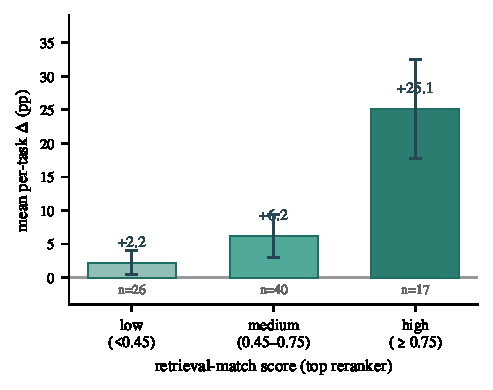
\includegraphics[width=\ifarxiv0.82\else0.5\fi\columnwidth]{figures/fig_coverage_binned.pdf}
\caption{Mean per-task SkillsBench gain by retrieval-match bin
(top reranker score of the best-matched skill, a proxy for corpus
coverage), pooled over the four cells, with $\pm$SE error bars.
The score is uncorrelated with the no-skill baseline, so the bins
are not a headroom artefact.  The per-task correlation and raw
scatter are in Appendix~\ref{app:coverage}.}
\label{fig:coverage-binned}
\end{figure}


